\documentclass[a4paper, 12pt]{article}

\usepackage[english]{babel}
\usepackage[utf8]{inputenc}
\usepackage[T1]{fontenc}
\usepackage{array}
\usepackage{fixltx2e}
\usepackage{amsmath}
\usepackage{amssymb}
\usepackage{graphicx}
\usepackage{caption}
\usepackage{float}
\usepackage{a4wide}
\usepackage{multicol}
\usepackage[table]{xcolor}
\usepackage{makeidx}
\usepackage{hyperref}
\usepackage{setspace}
\usepackage{indentfirst}
\usepackage[nottoc]{tocbibind}
\usepackage{listings}
\usepackage[font=footnotesize,labelfont=bf]{caption}
\usepackage[a4paper,top=1.60cm,bottom=1.60cm,left=1.37cm,right=1.45cm]{geometry}
\usepackage[square, sort, comma, numbers]{natbib}

\onehalfspacing
\graphicspath{{./img/}}
\makeindex

\usepackage{tikz}
\usetikzlibrary{calc,trees,positioning,arrows,chains,shapes.geometric,%
    decorations.pathreplacing,decorations.pathmorphing,shapes,%
    matrix,shapes.symbols}

\tikzset{
>=stealth',
  punktchain/.style={
    rectangle,
    rounded corners,
    draw=black, very thick,
    text width=8.3em,
    minimum height=1em,
    text centered,
    on chain},
  fillchain/.style={
    rectangle,
    rounded corners,
    fill=blue!30,
    draw=black, very thick,
    text width=8.3em,
    minimum height=1em,
    text centered,
    on chain},
  line/.style={draw, thick, <-},
  element/.style={
    tape,
    top color=white,
    bottom color=blue!50!black!60!,
    minimum width=4em,
    draw=blue!40!black!90, very thick,
    text width=8.3em,
    minimum height=1.5em,
    text centered,
    on chain},
  every join/.style={->, thick,shorten >=1pt},
  decoration={brace},
  tuborg/.style={decorate},
  tubnode/.style={midway, right=2pt},
}

\lstset{
    basicstyle=\scriptsize,
    morekeywords={either,or,transform,rule,to,from,through,function},
    frame=L,
}

\setcounter{secnumdepth}{2}
\setcounter{tocdepth}{2}

\begin{document}

\hypersetup{backref,pdfpagemode=FullScreen,colorlinks=true}

\thispagestyle{empty}
\begin{center}
    \vspace*{4cm}
    \textbf{\Large{An Introduction to the Autotuning\\of Parallel Applications}}\\

    \vskip 1cm

    Pedro \textsc{Bruel}

    \emph{phrb@ime.usp.br}

    \vfill
    \normalsize{\emph{DCC - IME\\
    Universidade de São Paulo}\\}
    \normalsize{São Paulo, \today}
\end{center}

\newpage

\tableofcontents

\newpage

\section{Introduction} \label{sec:intro}

A number of factors make programming \textbf{H}igh-\textbf{P}erformance
\textbf{C}omputing applications a very complex task. To achieve high
performance it is necessary to write programs that take into consideration
the specifics of a parallel architecture, as well as the basic concepts
of parallel programming. Parallel computing platforms are increasingly
available and heterogeneous. Processors are now expected to be multi-core,
and even personal computers have coprocessors and accelerators such as
GPUs. Consequently, it is easy to over-optimize a parallel program to
a specific parallel computing platform.

This leads to highly efficient hand-optimized programs, capable of leveraging
the potential of a specific parallel computing platform. Although, despite the
efforts made during implementation, this highly-optimized program will not able
to achieve the same performance in a different parallel architecture. In other
words, the performance achieved by extensive hand-optimization is
not \emph{portable}. The lack of performance portability of HPC applications,
as well as the immense efforts needed to optimize them, justify the research
for automated methods of optimization for parallel programs.

Extensive research in the last decade produced powerful tools for
automatically tuning programs, or \emph{autotuners}, in a variety of problem
domains. Despite being able to achieve good results on porting the performance
of parallel programs,these tools are not widely utilized by the scientific
and programming communities, perhaps because of their novelty.

Autotuners can be model-based or empirical. Model-based autotuners predict
program performance following a model of the target architecture. The model
is built previous to the tuning and execution, during an \emph{installation}
phase. Empirical autotuners discover the best optimization of a program by
executing different optimized versions and measuring their performance. No
model is built or used, instead empirical autotuner commonly use search
techniques to explore the space defined by the possible optimizations
of a program, in a given architecture. Despite being arguably slower than
model-base autotuners, given a model is already built, empirical autotuners
can produce optimized versions of a program during tuning time. The empirical
tuning strategy allows programmers to focus their efforts in designing
programs that explicitly expose their implementation and optimization choices,
leaving the task of discovering the best choice to the autotuner.

The search techniques used by an autotuner can target the optimization of
various program metrics. Simple metrics such as runtime can be obtained by
simply running the candidate optimization, but more complex metrics, such
as I/O patterns or memory accesses are not so straight-forward to measure.
\emph{Profilers} are tools that offer such specific measurements and analysis
of programs during runtime. For instance, if a programmer was interested in
optimizing the CPU load, or the duration and depth of a function call stack
during the execution of her program, she could use a profiler to produce such
measurements to an empirical autotuner.

This Introduction to Parallel Tuning aims to familiarize the reader with the
state-of-the-art applications of autotuning techniques to the optimization
of high-performance parallel programs. The following section discuss the
autotuning technique under the Algorithm Selection framework. Section
\ref{sec:insieme} discusses the INSIEME compiler project for parallel
applications. Section \ref{sec:opentuner} describes the OpenTuner framework,
an autotuning framework that can be used to implement autotuners for parallel
applications. Section \ref{sec:profilers} list some profiling tools that can
be used to measure metrics of parallel programs. Section \ref{sec:related}
discusses some of the recent work on parallel automatic optimization.
Finally, section \ref{sec:conclusion} summarizes the discussion.

\section{Autotuning} \label{sec:autotuning}

The idea behind empirical autotuning techniques consists of using the
performance-impacting features of architectures, problems and algorithms
in a domain to define sets of possible algorithm implementations,
configurations and optimizations. These sets describe a \emph{search space}
that can then be explored by searching, optimization and Machine Learning
techniques.

In contrast, model-based autotuning uses perfomance-impacting features
to build a model, and then uses this model to autotune an application.
The model can be obtained by formally describing an algorithm and analysing
its behaviour or, when building a model for a computer architecture,
empirically exploring the search space.
Models are then used to implement highly optimized libraries for a given
domain, that are then used to implement programs in that domain. Different
compiled versions of the library functions must be provided for all target
architectures.

Instead of manually exploring the search space of algorithm optimizations,
configurations and implementations, programmers should be motivated to expose
these features to an autotuner. This approach to designing and implementing
computer programs is called \emph{Programming by Optimization}, and was
first described by Hoos~\cite{hoos2012programming}.

Autotuning techniques have been used since as early as 1997, when the PHiPAC
system~\cite{bilmes1997phipac} used code generators and search scripts to
automatically generate high performance code for matrix multiplication. Since
then the autotuning problem has been tackled in multiple domains, with a great
variety of strategies. Whaley \emph{et al.}~\cite{whaley1998atlas} introduce the
ATLAS project, that produced optimized dense matrix multiply routines. The
OSKI~\cite{vuduc2005oski} library provides automatically tuned kernels for
sparse matrices. The FFTW~\cite{frigo1998fftw} library provides tuned C
subroutines for computing the Discrete Fourier Transform.

More recently, there have been efforts in the direction of breaking the domain
boundaries, through the implementation of tools that generalize autotuning.
PetaBricks~\cite{ansel2009petabricks} is a language, compiler and autotuner for
domain-independent applications, that introduce new abstractions such as the
\emph{either...or} keywords, which let programmers define multiple algorithms
for a same problem. The user can define \emph{input
features}~\cite{ding2014autotuning} for a given algorithm, which allow
Petabricks to group and specifically optimize programs for classes of
training inputs.

The OpenTuner framework~\cite{ansel2014opentuner} implements ensembles of search
techniques that are used to search a user-defined space of program
configurations. OpenTuner is further discussed in section~\ref{sec:opentuner}.
The framework has already been used to implement a domain specific language
for data-flow programming \cite{bosboom2014streamjit}
and a framework for the optimization of recursive parallel
algorithms~\cite{eliahu2015frpa}. The ParamILS
framework~\cite{hutter2009paramils} implements state-of-the-art search methods
for algorithm configuration and parameter tuning.

In an effort to provide a common representation of multiple parallel
programming models, the INSIEME compiler project~\cite{jordan2012multi}
implements abstractions for OpenMP, MPI and OpenCL. The INSIEME compiler is
able to generate optimized parallel code for heterogeneous multi-core
architectures. Section~\ref{sec:insieme} discusses the INSIEME compiler project.

The remaining of this section presents the \emph{Algorithm Selection Problem}
and describes autotuning as an instance of this problem.

\subsection{The Algorithm Selection Problem}

\begin{figure}[H]
    \centering
    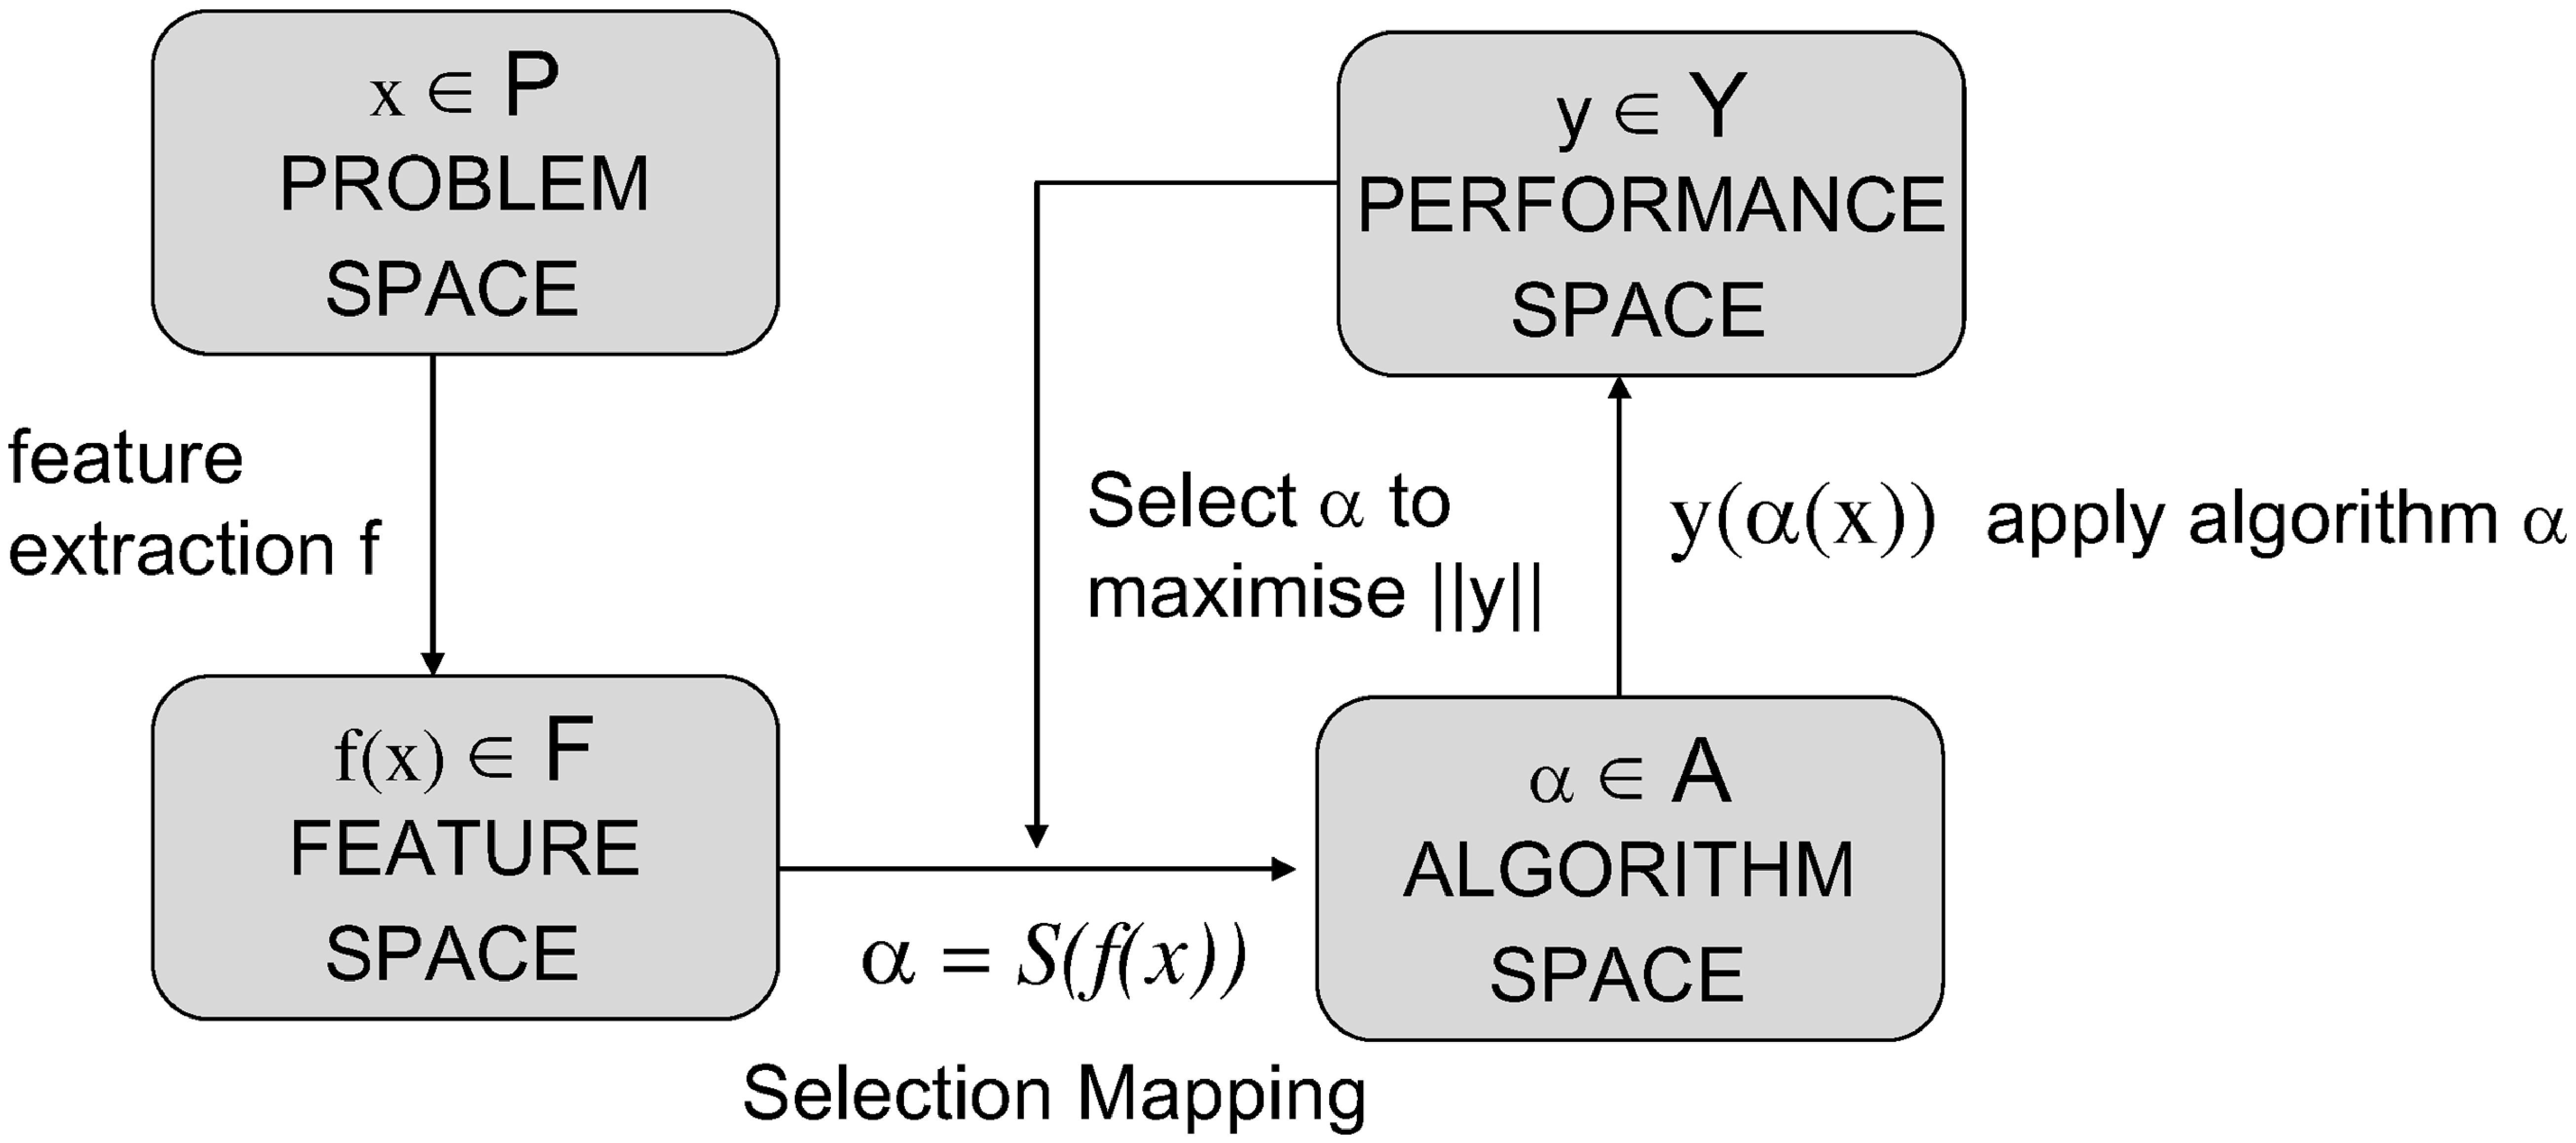
\includegraphics[width=0.45\textwidth]{algoselframe}
    \captionsetup{width=0.64\textwidth}
    \caption{Schematic diagram of the Algorithm Selection Problem as described by~\citet{rice1976algorithm}. Reproduction of a diagram from~\citet{smith2008cross}.}
    \label{fig:algoselframe}
\end{figure}

The description of the Algorithm Selection Problem was first published by Rice
in 1976~\cite{rice1976algorithm}. The problem is described as follows.  Given a
set $A$ of \emph{algorithms}, a set $P$ of \emph{problems} and a set $F$ of
\emph{problem features}, the Algorithm Selection Problem consists of finding a
\emph{mapping} of algorithms to problems that minimizes the time to solve all
problems in the set, taking problem features in consideration. The
\emph{performance space} $Y$ is composed of the measurements of each algorithm
$\alpha \in A$ in each problem $x \in P$. 

Note that the \emph{algorithms} that compose a set are not limited to
configurations or combinations of algorithms. Each $\alpha \in A$ can represent
different abstractions, such as programs, heuristics, or configurations. The
set of \emph{problems} usually contains instances of a problem, and the set of
\emph{problem features} contains representations of the performance-impacting
features. \citet{ding2014autotuning} further discusses the feature extraction
processes.  Figure \ref{fig:algoselframe} shows a schematic diagram for the
Algorithm Selection Problem, as described by Rice.

\citet{kotthoff2012algorithm} presents a survey of the algorithm selection
field and its applications in combinatorial search problems.
\citet{smith2008cross} surveys the applications of the algorithm selection
problem to the machine learning and meta-learning fields.

The Algorithm Selection Problem is hard. Its NP-completeness has been proved
when calculating static distributions of algorithms in parallel machines
\cite{bougeret2009combining}. Its Undecidability in the general case was also
shown~\cite{guo2003algorithm}. Therefore, methods such as \emph{Stochastic
Local Search} can be used to approach the algorithm selection problem with good
results, as described by~\citet{hutter2009paramils}.

\subsection{INSIEME Compiler Project} \label{sec:insieme}

The INSIEME Compiler Project\footnote{insieme-compiler.org} of the University 
of Innsbruck is a C/C++ source-to-source compiler that aims to automatically 
optimize parallel programs for heterogeneous parallel computing platforms, 
regardless of the parallel programming tools used in the implementation of 
the programs.

INSIEME~\cite{jordan2012multi} uses the INSPIRE intermediate
representation~\cite{jordan2013inspire} to commonly represent
parallel programs in various parallel programming abstractions,
such as OpenMP, MPI and OpenCL. INSIEME also offers a runtime
system for online tuning and performance monitoring.

An overview of the architectures of the INSIEME compiler and runtime
systems is presented in Figures \ref{fig:insiemearch} and \ref{fig:insiemerun}.
Those diagrams can be found at the INSIEME Compiler Project 
website\footnote{insieme-compiler.org/architecture.html}.

\begin{figure}[H]
    \centering
    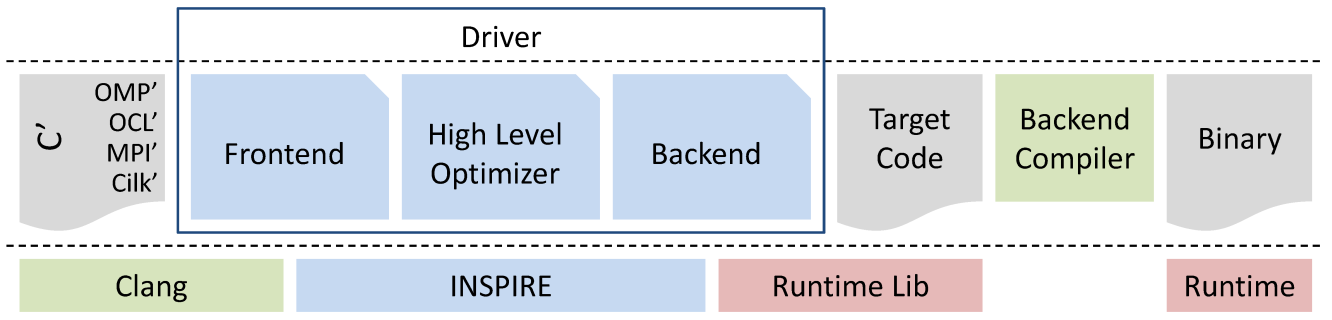
\includegraphics[width=0.63\textwidth]{architecture_compiler}
    \captionsetup{width=0.64\textwidth}
    \caption{Overview of the INSIEME compiler.}
    \label{fig:insiemearch}
\end{figure}

\begin{figure}[H]
    \centering
    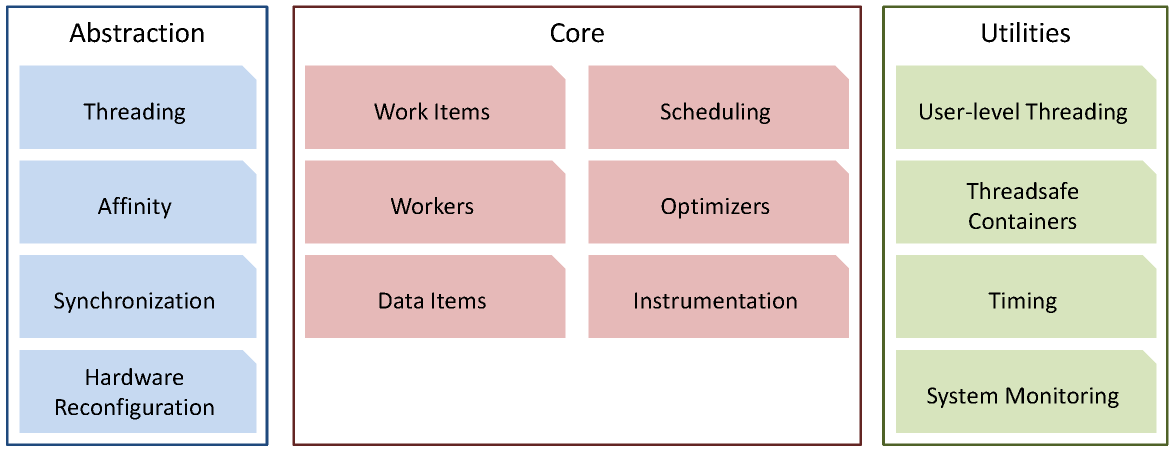
\includegraphics[width=0.63\textwidth]{architecture_runtime}
    \captionsetup{width=0.64\textwidth}
    \caption{Overview of the INSIEME runtime.}
    \label{fig:insiemerun}
\end{figure}

The runtime uses multiple threads to schedule and distribute work. The
optimization and scheduling choices are made based on previous executions
of the program and on knowledge of the underlying parallel computing
platform.

\subsection{OpenTuner Framework} \label{sec:opentuner}

The OpenTuner framework~\cite{ansel2014opentuner} provides domain-agnostic
tools for defining search spaces and implementing autotuners.

The search spaces are defined by instantiating the different 
\emph{Parameter} types provided by the framework. Each parameter
type, such as \emph{FloatParameter}, \emph{IntegerParameter} or
\emph{BooleanParameter} implements its own manipulation functions,
that allow the search techniques to navigate the values allowed
to each parameter, thus exploring the search space defined by the
user. A user of the framework can implement her own
parameter types.

OpenTuner implements ensembles of optimization and Machine 
Learning techniques that perform well in different problem domains,
and are used to search user-defined search spaces. The results found
during the search process are shared between techniques through a
common results database.
OpenTuner uses \emph{meta-techniques} for coordinating the
distribution of resources between techniques in an ensemble.

An OpenTuner application can implement its own search techniques and
meta-techniques, adding them to existing ensembles or creating completely
new ones.
By separating search space definition from search method implementation,
OpenTuner allows fast implementation of autotuners for different
problem domains.

The search techniques implemented in OpenTuner share the results found
through a common database. This allows techniques to benefit from each
other's executions and reach better results faster.

Figure~\ref{fig:opentuner} illustrates the main components of the framework,
the interactions between them.

\begin{figure}[H]
    \centering
    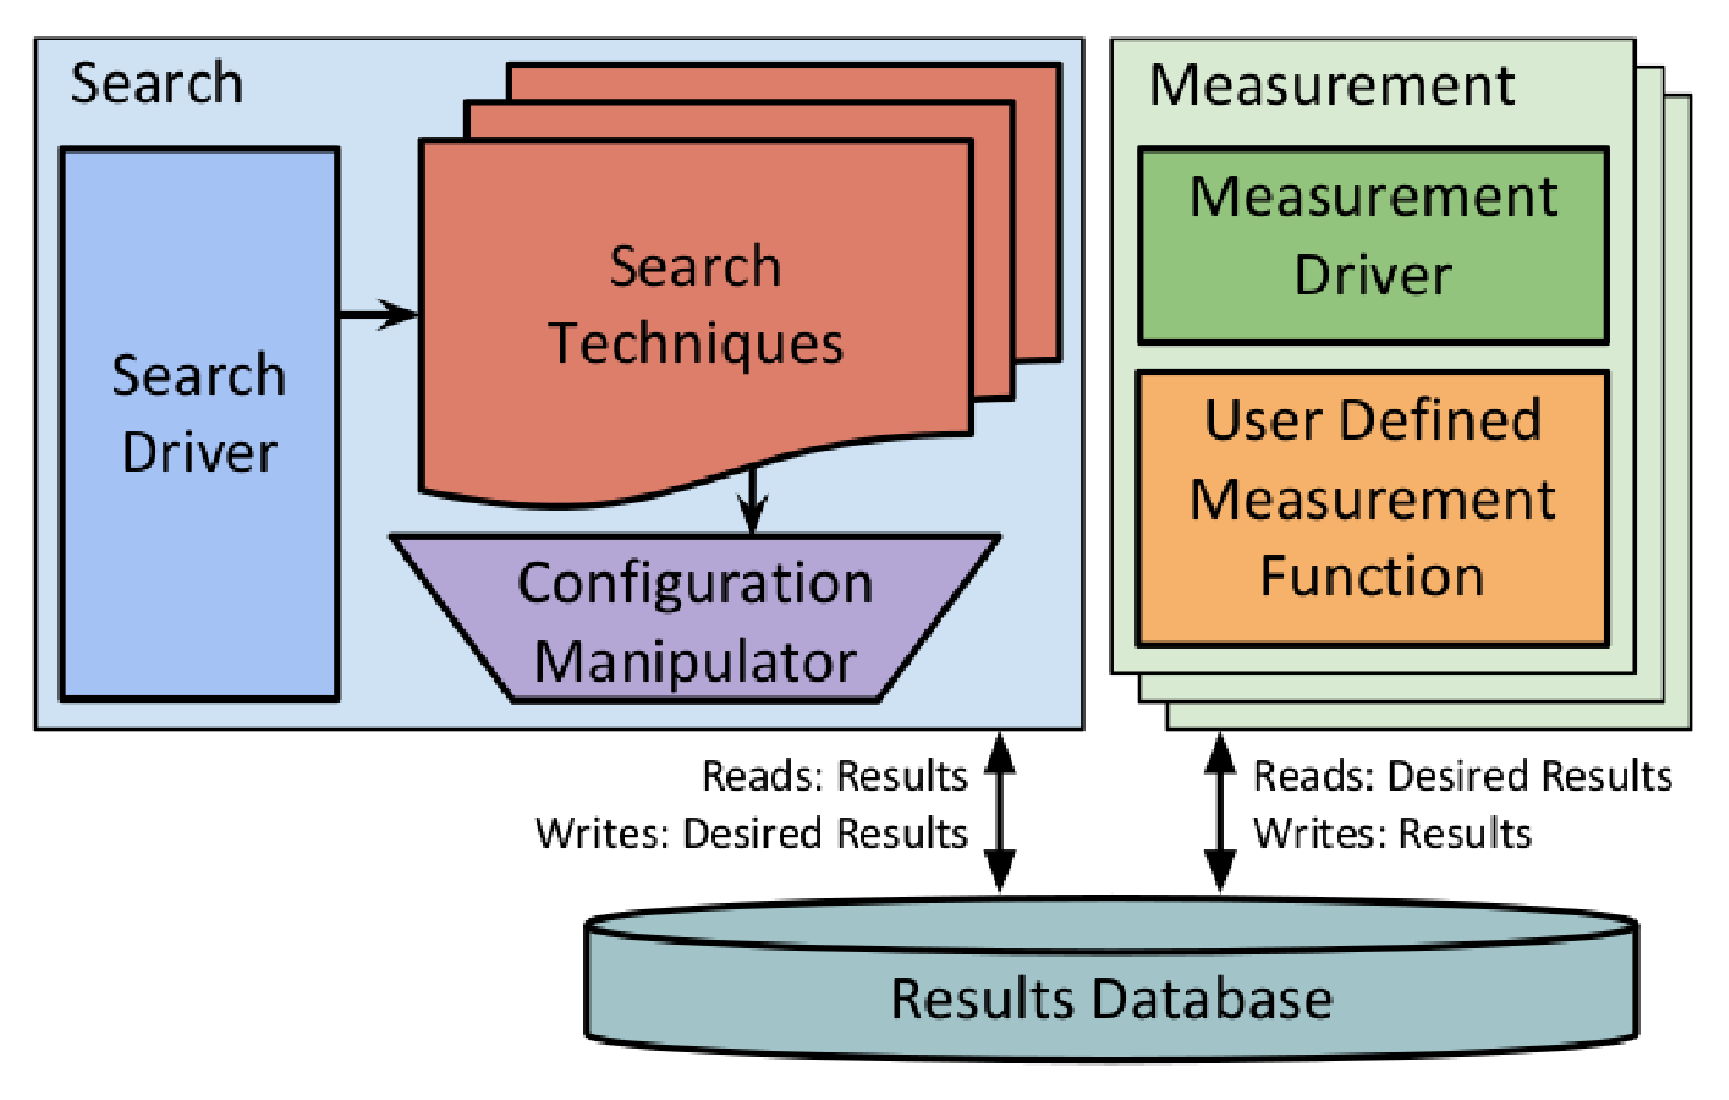
\includegraphics[width=0.45\textwidth]{opentuner}
    \captionsetup{width=0.64\textwidth}
    \caption{Main components of the OpenTuner framework and their interations. Reproduction of a diagram found in~\citet{ansel2014opentuner}.}
    \label{fig:opentuner}
\end{figure}

\section{Profiling Tools} \label{sec:profilers}

- Add table of parallel and GPU profilers.

\section{Related Work} \label{sec:related}

\subsection{FRPA}

\subsection{GPU tunning*}

\subsection{Compiler Parameters*}

\section{Conclusion} \label{sec:conclusion}

\bibliographystyle{plainnat} 
\bibliography{Introduction_to_Parallel_Tuning}

\end{document}
